\documentclass[11pt,compress,t,notes=noshow, aspectratio=169, xcolor=table]{beamer}
\usepackage{../../style/lmu-lecture}
% This file is included in slides and exercises

% Rarely used fontstyle for R packages, used only in 
% - forests/slides-forests-benchmark.tex
% - exercises/single-exercises/methods_l_1.Rnw
% - slides/cart/attic/slides_extra_trees.Rnw
\newcommand{\pkg}[1]{{\fontseries{b}\selectfont #1}}

% Spacing helpers, used often (mostly in exercises for \dlz)
\newcommand{\lz}{\vspace{0.5cm}} % vertical space (used often in slides)
\newcommand{\dlz}{\vspace{1cm}}  % double vertical space (used often in exercises, never in slides)
\newcommand{\oneliner}[1] % Oneliner for important statements, used e.g. in iml, algods
{\begin{block}{}\begin{center}\begin{Large}#1\end{Large}\end{center}\end{block}}

% Don't know if this is used or needed, remove?
% textcolor that works in mathmode
% https://tex.stackexchange.com/a/261480
% Used e.g. in forests/slides-forests-bagging.tex
% [...] \textcolor{blue}{\tfrac{1}{M}\sum^M_{m} [...]
% \makeatletter
% \renewcommand*{\@textcolor}[3]{%
%   \protect\leavevmode
%   \begingroup
%     \color#1{#2}#3%
%   \endgroup
% }
% \makeatother

\title{Interpretable Machine Learning}
\date{}
\begin{document}
\lecturechapter{Shapley Values}
\lecture{Interpretable Machine Learning}


\begin{vbframe}{Shapley Values}
Shapley values are a concept of \textbf{cooperative game theory}:
\begin{itemize}
  \item In cooperative games, a set of players $P$ with $P = \{1, \hdots, p\}$ forms a coalition $S \subseteq P$.
  \item A value function $v(S)$ describes the payout (or gain) achieved by the coalition $S$.
  \item As some players contribute more than others, we are interested in the distribution of the payout among the players.
  \item We can measure the payout of each player by Shapley values.
  \item The \textbf{Shapley value} assigns a value to each player according to the marginal contribution of each player in all possible coalitions.
\end{itemize}
\end{vbframe}

\begin{vbframe}{Shapley Values}
In Machine Learning, we can use Shapley values to explain individual predictions of specific observations:
\begin{itemize}
  \item Players $\hat{=}$ features.
  \item Features collaborate to make a prediction.
  \item The payout of coalition $S$ for observation $\xv$ is
  $$v(\xv_S) =  \fh_{S} (\xv_S) - \E (\fh(\xv))$$
  i.e., the difference of the marginal prediction of $\xv_S$ and the average prediction.
  \item We have already seen how the marginal prediction can be calculated: ICE curves.
\end{itemize}
\begin{center}
\vspace{-0.3cm}
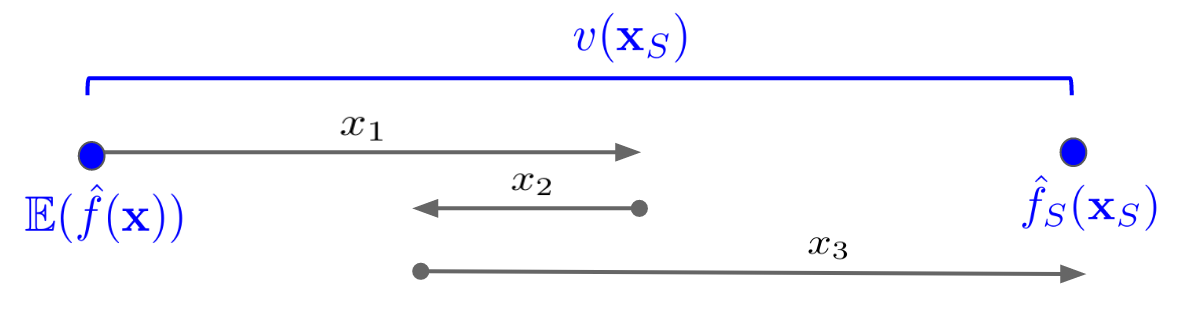
\includegraphics[width=0.8\textwidth]{figure_man/shapley_valuefct}
\end{center}
\end{vbframe}

\begin{vbframe}{Shapley Values}

\begin{itemize}
 \item Shapley values tell us what the payout of each feature is, i.e., how each feature contributes to the overall prediction of a specific observation.
    \item The Shapley value is the average marginal contribution of a feature towards the prediction \textbf{across all possible feature coalitions}.
    \item The sum of Shapley values over all features yields the difference between the average prediction of all data points (baseline) and the selected individual prediction.
  \end{itemize}
\end{vbframe}

\frame{
\frametitle{Shapley Values - Illustration}
The Shapley value of the feature $x_2$ is the marginal contribution (prediction change) when $x_2$ enters an abitrary coalition. \\
\only<1>{Here, $x_2$ enters the coalition secondly, resulting in a prediction change of $24-12 = 12$. Overall, the coalition increases the prediction by 36.}
\only<2>{We produce all possible orders of feature coalitions and measure the prediction change if feature $x_2$ enters the coalition.}
\begin{center}
  \only<1>{
    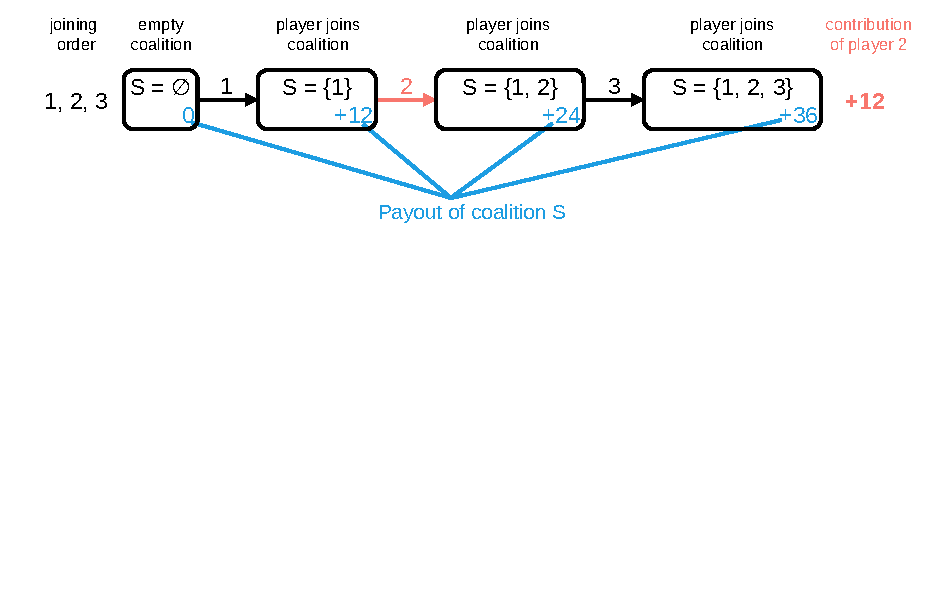
\includegraphics[page=1, width=0.6\textwidth]{figure_man/shapley_feature_effect}
  }
  \only<2>{
    \includegraphics[page=2, width=0.6\textwidth]{figure_man/shapley_feature_effect}
  }
\end{center}

}


\begin{vbframe}{Shapley Value - Definition}
\begin{itemize}
  \item The Shapley value of a feature $j$ is defined as:\\
  For $m = 1, \dots, M$ exhaustively select coalition $S_m \subseteq P \land S_m \backslash j$  and calculate
$$ \hat{\phi_{j}}(\xv) = \frac{1}{M} \sum_{m=1}^{M} \underbrace{v(\xv_{S_m \cup \{j \} }) - v(\xv_{S_m})}_{\text{marginal contribution of feature $j$}} $$
\lz
  \item Interpretation of Shapley value $\hat{\phi_{j}}(\xv)$ for feature $j$ and observation $\xv$:
  The feature value $\xv_{j}$ contributed $\hat{\phi_{j}}(\xv)$ towards the prediction $\fh(x)$ compared to the average prediction for the dataset.
\end{itemize}
\lz
\tiny
Shapley, Lloyd S. 1953. $"$A Value for N-Person Games.$"$\\
\vspace{0.2cm}
Strumbelj, Erik, Igor Kononenko, Erik Strumbelj, and Igor Kononenko. 2014. $"$Explaining prediction models and individual predictions with feature contributions.$"$

\end{vbframe}

\begin{vbframe}{Bike Sharing Dataset}

\begin{center}
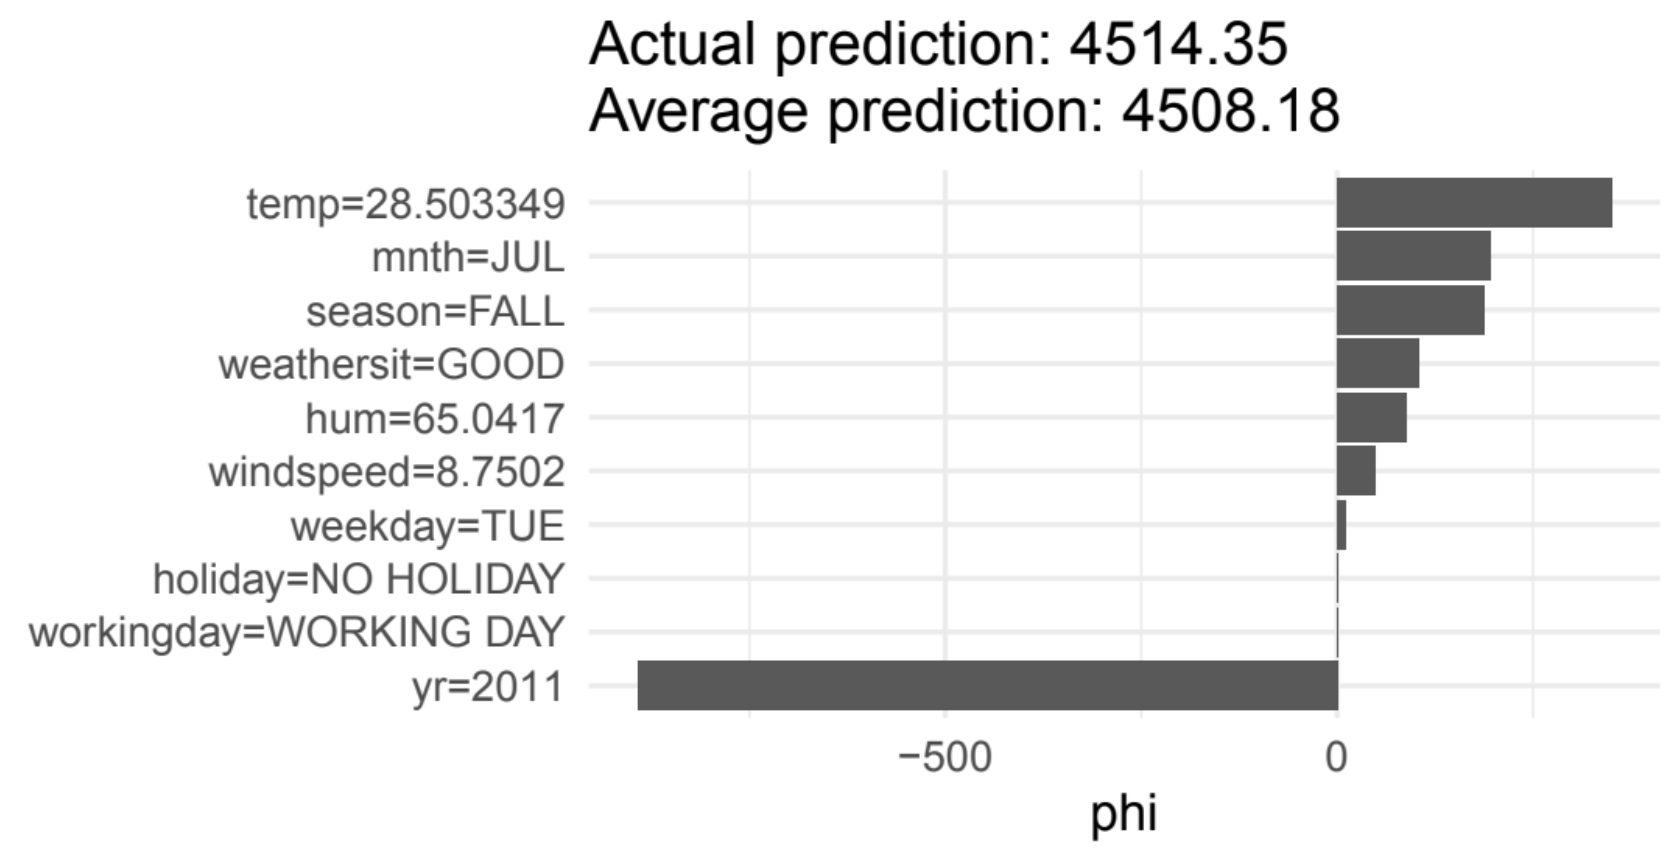
\includegraphics[width=0.65\textwidth]{figure_man/bike-sharing03.png}
\end{center}

The plot shows the Shapley values for observation 200.
The difference between the model prediction of this observation and the average prediction of the data is fairly distributed among the features (i.e., 4514 - 4508).
The most positive effect had feature value temp=28.503349, with a contribution (increase of prediction) of + 350.
\end{vbframe}


\endlecture
\end{document}
